\section{Project Background}

\subsection{Wireless Sensor Networks}
Wireless Sensor Networks (WSNs) are simple, low-cost networks that primarily consist of nodes and a base station \cite{WSN-WaterQual}. WSN nodes usually comprise of some sensing or measuring capability acting as the physical layer, and relay this information via uplink to a base station for processing and then to a network server acting as the network layer. From here, the API from a network cloud service can be used to create GUI's and other applications for researchers and consumers which acts as the application layer. 

Innovating many field of industry and research, these distributed networks of nodes have been valuable in many contexts. For example, the use of ZigBee communication technology for air pollution monitoring \cite{ZigBeeAirPolution} and the use of Bluetooth for communication between end-devices measuring temperature, luminance, carbon dioxide and humidity for energy-saving establishments \cite{BTenergySaving}. Although these WSNs have worked in the past, the future of this technology lies in developing systems that have high scalability and range, something that ZigBee and Bluetooth inherently lack. Cellular and satellite technology are alternate approaches that offer extremely high data rates and range, however these technologies are not practical to implement in most situations due to exceedingly high costs. 

\subsection{Structural Health Monitoring}
Structural Health Monitoring (SHM) is a vital practice for ensuring the safety and longevity of civil and industrial structures \cite{SHM-IoT-Magazine}. SHM involves continuously tracking change in structures which can be attributed to material aging, environmental influences or unforeseen incidents such as traffic accidents or natural disasters. These changes can be tracked using WSNs equipped with appropriate sensor modules, and integrating data transmission capabilities. A survey investigating the implementation of IoT technology for structural health monitoring (SHM) determined that WSN technology has revolutionized the health monitoring in various fields including civil engineering \cite{SHM-IoT-Survey}. WSN  systems can be deployed to measures a vast array of SHM indicators including temperature, velocity, acceleration, frequency and displacement. WSN can be deployed on a structure such as a bridge operating as Internet of Things (IoT) nodes. This deployment highlights the advantage of using WSNs for SHM since the collected data can be uploaded to the cloud for processing and distribution. Within the context of bridge monitoring, the integration of WSN with IoT for SHM can serve various application requirements for real-time data uplink such as monitoring acceleration and frequency characteristics. This data can be plotted on a continuous time spectrum and compared to observational data such as pedestrian load to verify the validity of  simulated truss analysis models and finite elements (FE) simulation. 

\subsection{Internet of Things}
The Internet of Things (IoT) is an `interconnected network of things' \cite{IoT}, where `things' in this context is defined as an end-device with WSN type capability. The IoT architecture comprises of six-layers, the coding layer, perception layer, network layer, middle-ware layer, application layer and business layer \cite{IoT}. Thus to create this IoT architecture for research purposes the first five layers need to be implemented. LoRa end-devices act as the physical layer encompassing the coding and perception layer. The coding layer involves associating unique ID specifiers to each end device \cite{IoT} and the perception layer is involved with on-board sensing and data acquisition. The network layer is a relay of this perceptual information to a gateway, and the middle-ware layer is the IoT cloud platform that facilitates these connections and receives information from the network layer. The application layer involves pulling the API or information from the network layer and developing apps or graphical user interfaces (GUIs) to display the data.\\\\
The Things Network (TNN) is an open-source LoRaWAN network server used to construct IoT cloud applications with end-to-end encryption and secure communication \cite{LoRaWAN-Smart-Infrastructure-Monitoring}. TNN exists on the middle-ware layer and can be used to deploy an IoT architecture using LoRa end-devices in the coding and perception layer, and utilize the LoRaWAN communication protocol in the network layer. TNN offers a console and API to develop applications that serve as the architecture's application layer. Figure \ref{LoRa-IOT-Example} displays an example of an IoT architecture using WSN nodes, a LoRaWAN gateway, cloud storage and user devices. 

\begin{figure}[h]
	\centering
	\caption{The LoRa network architecture for agriculture area. \cite{LoRaWAN-WSN-Agricultual-Application}}
	\label{LoRa-IOT-Example}
	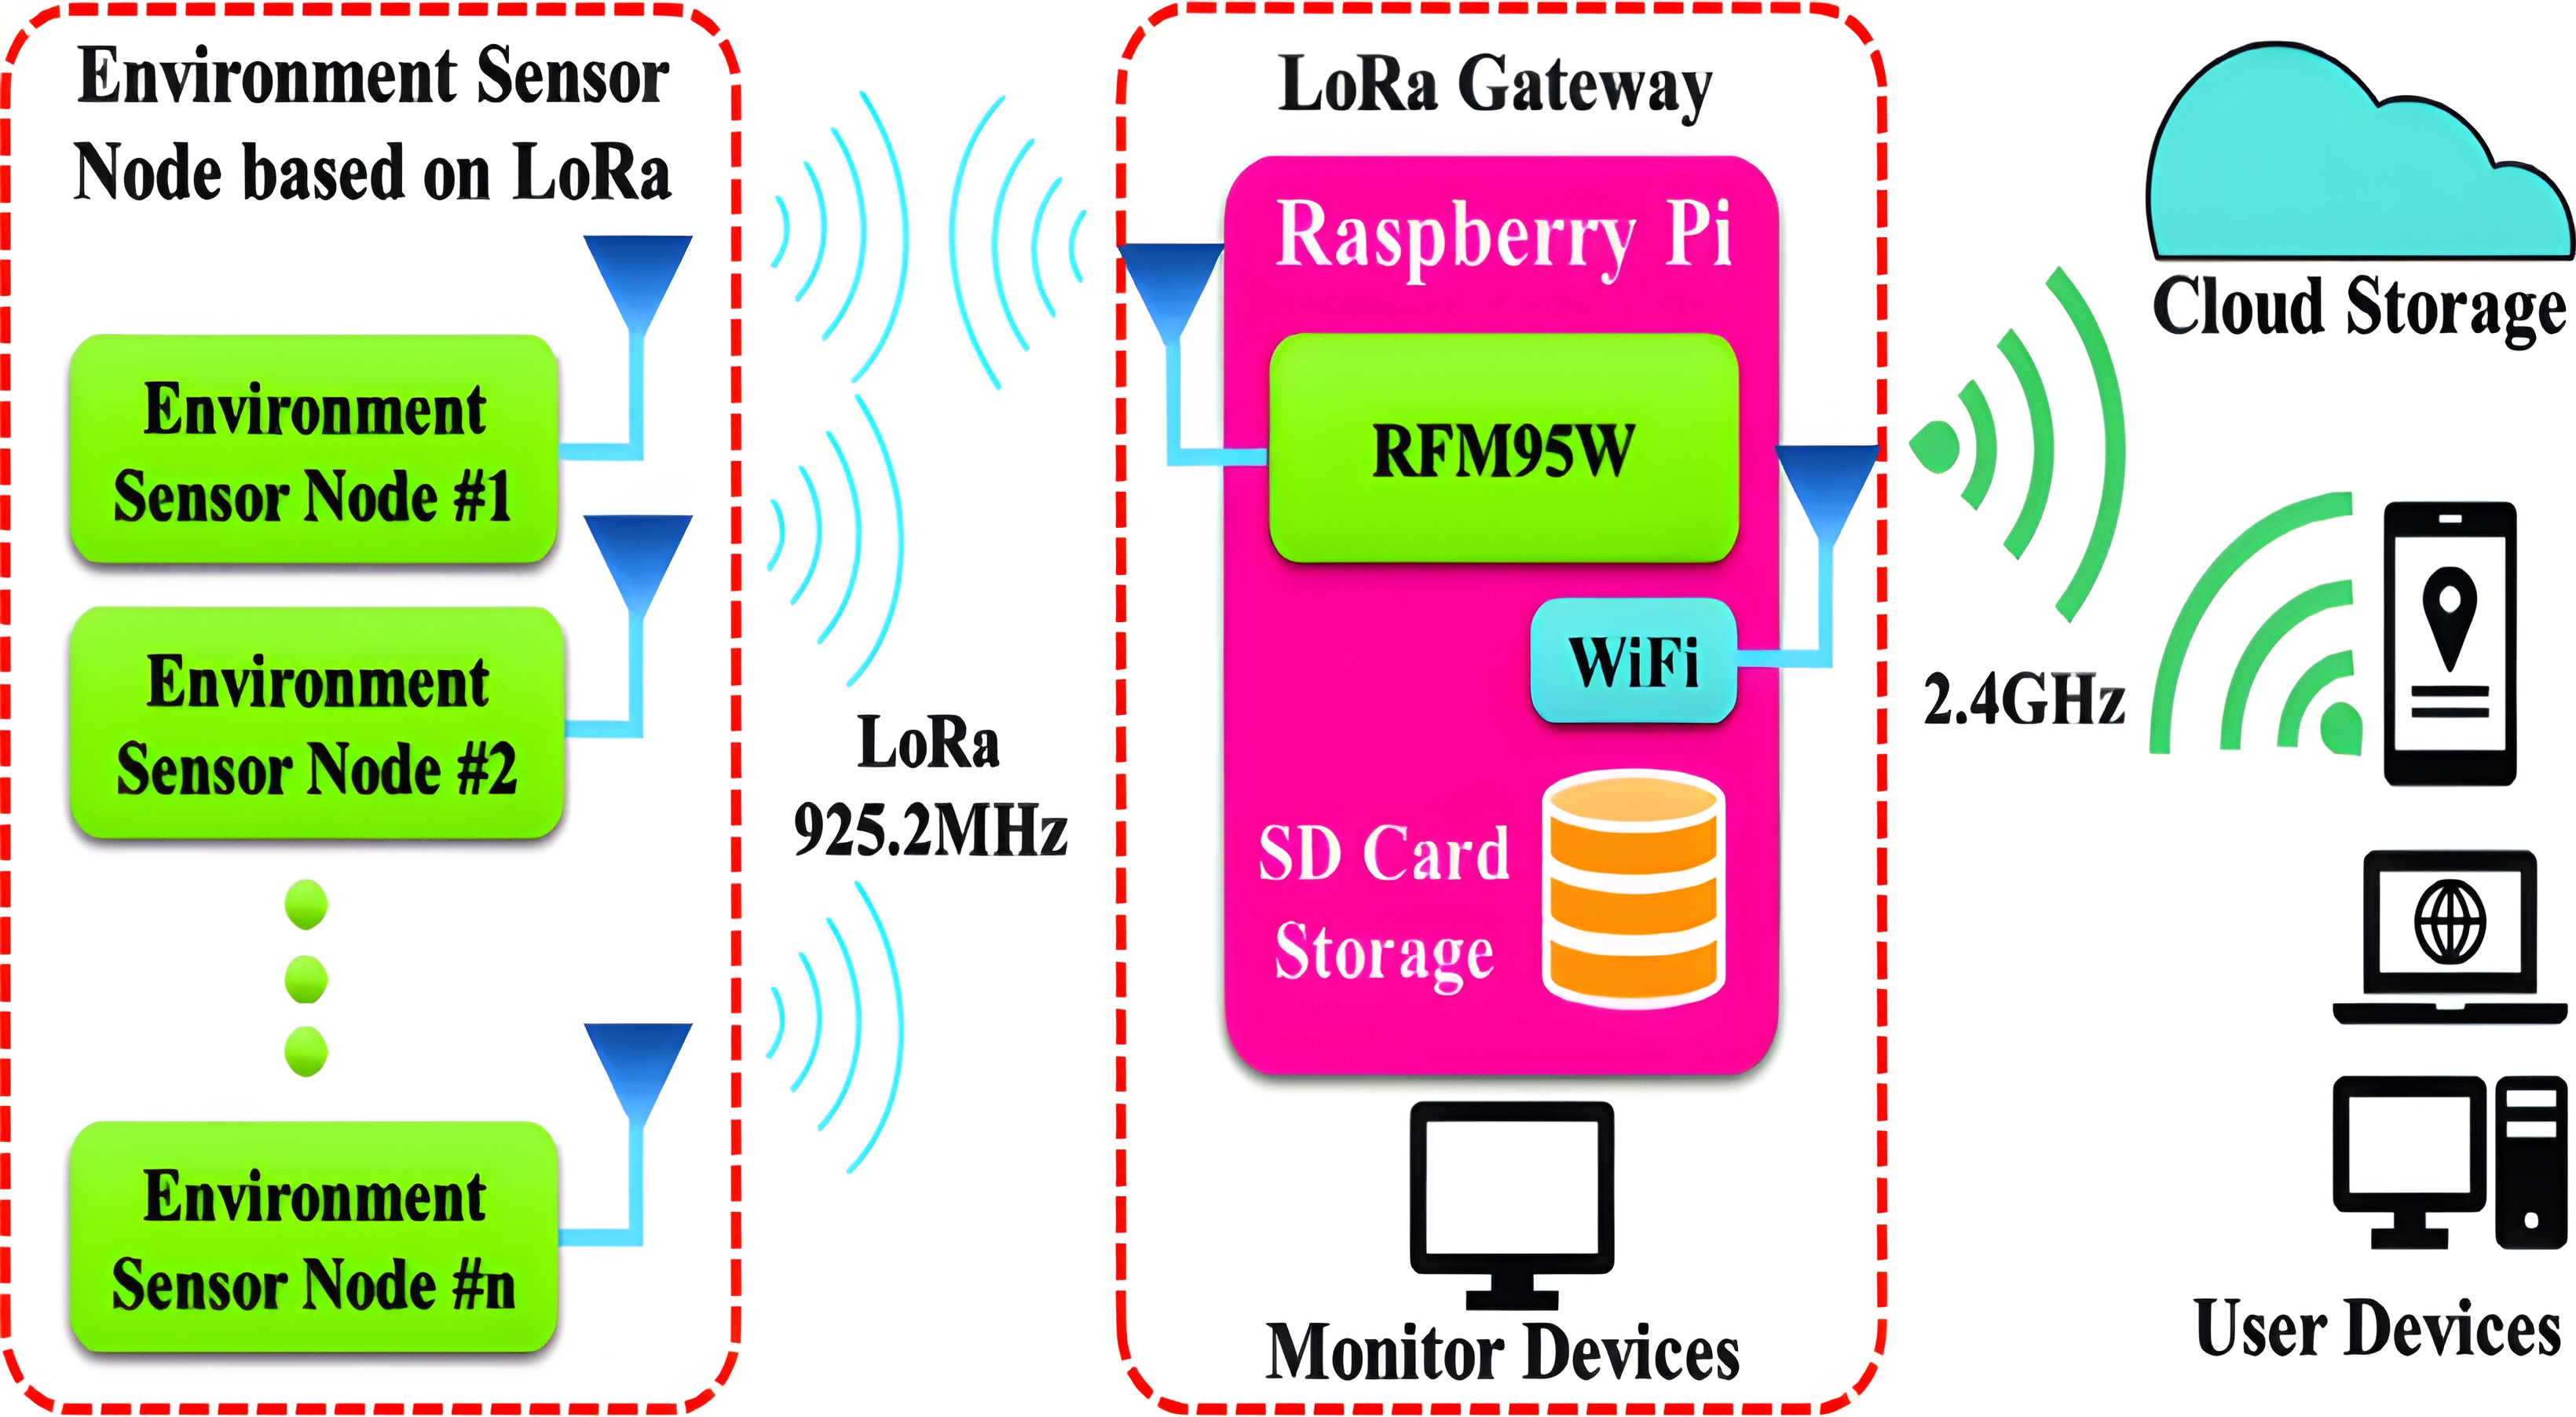
\includegraphics[scale=0.1]{Sections/Introduction/LoRaWAN-IOT-Example.jpg}
\end{figure}


\subsection{LoRa and LoRaWAN}
Low Power Wide Area Network (LPWAN) is a communication technology that offers wide coverage, similar to satellite networks, while maintaining lower data rates akin to ZigBee. The technology is distinguished by its ultra-low power consumption and cost-effective deployment and maintenance  \cite{IOTandLORAWAN-SmartFarm}.\\\\
LoRa and LoRaWAN, forms of LPWAN technology, were developed to overcome the scalabilty issues associated with traditional WSN configurations that relied on short-range communication protocols such as Zigbee and Bluetooth \cite{WSN-WaterQual}. These configurations often used a mesh network layout, which introduced challenges in network management and power consumption with increasing network size \cite{IOTandLORAWAN-SmartFarm}.\\\\
LoRaWAN's unique `star of stars' configuration addresses these challenges by enabling scalable network expansion with reduced complexity. LoRa itself is a Chirp Spread Spectrum (CSS) modulation technique developed by Cycleo, offering a Medium Access Control (MAC) protocol and operating on license-free, region-dependent Industrial, Scientific and Medical (ISM) frequency bands \cite{IOTandLORAWAN-SmartFarm}.

\begin{comment}
\begin{figure}[h]
	\centering 
	\caption{Comparison of main IoT enabling communication technologies in terms of range, data rate, energy consumption, and costs. \cite{IOTandLORAWAN-SmartFarm}}
	\label{IOTandLORAWAN-SmartFarm-Figure1}
	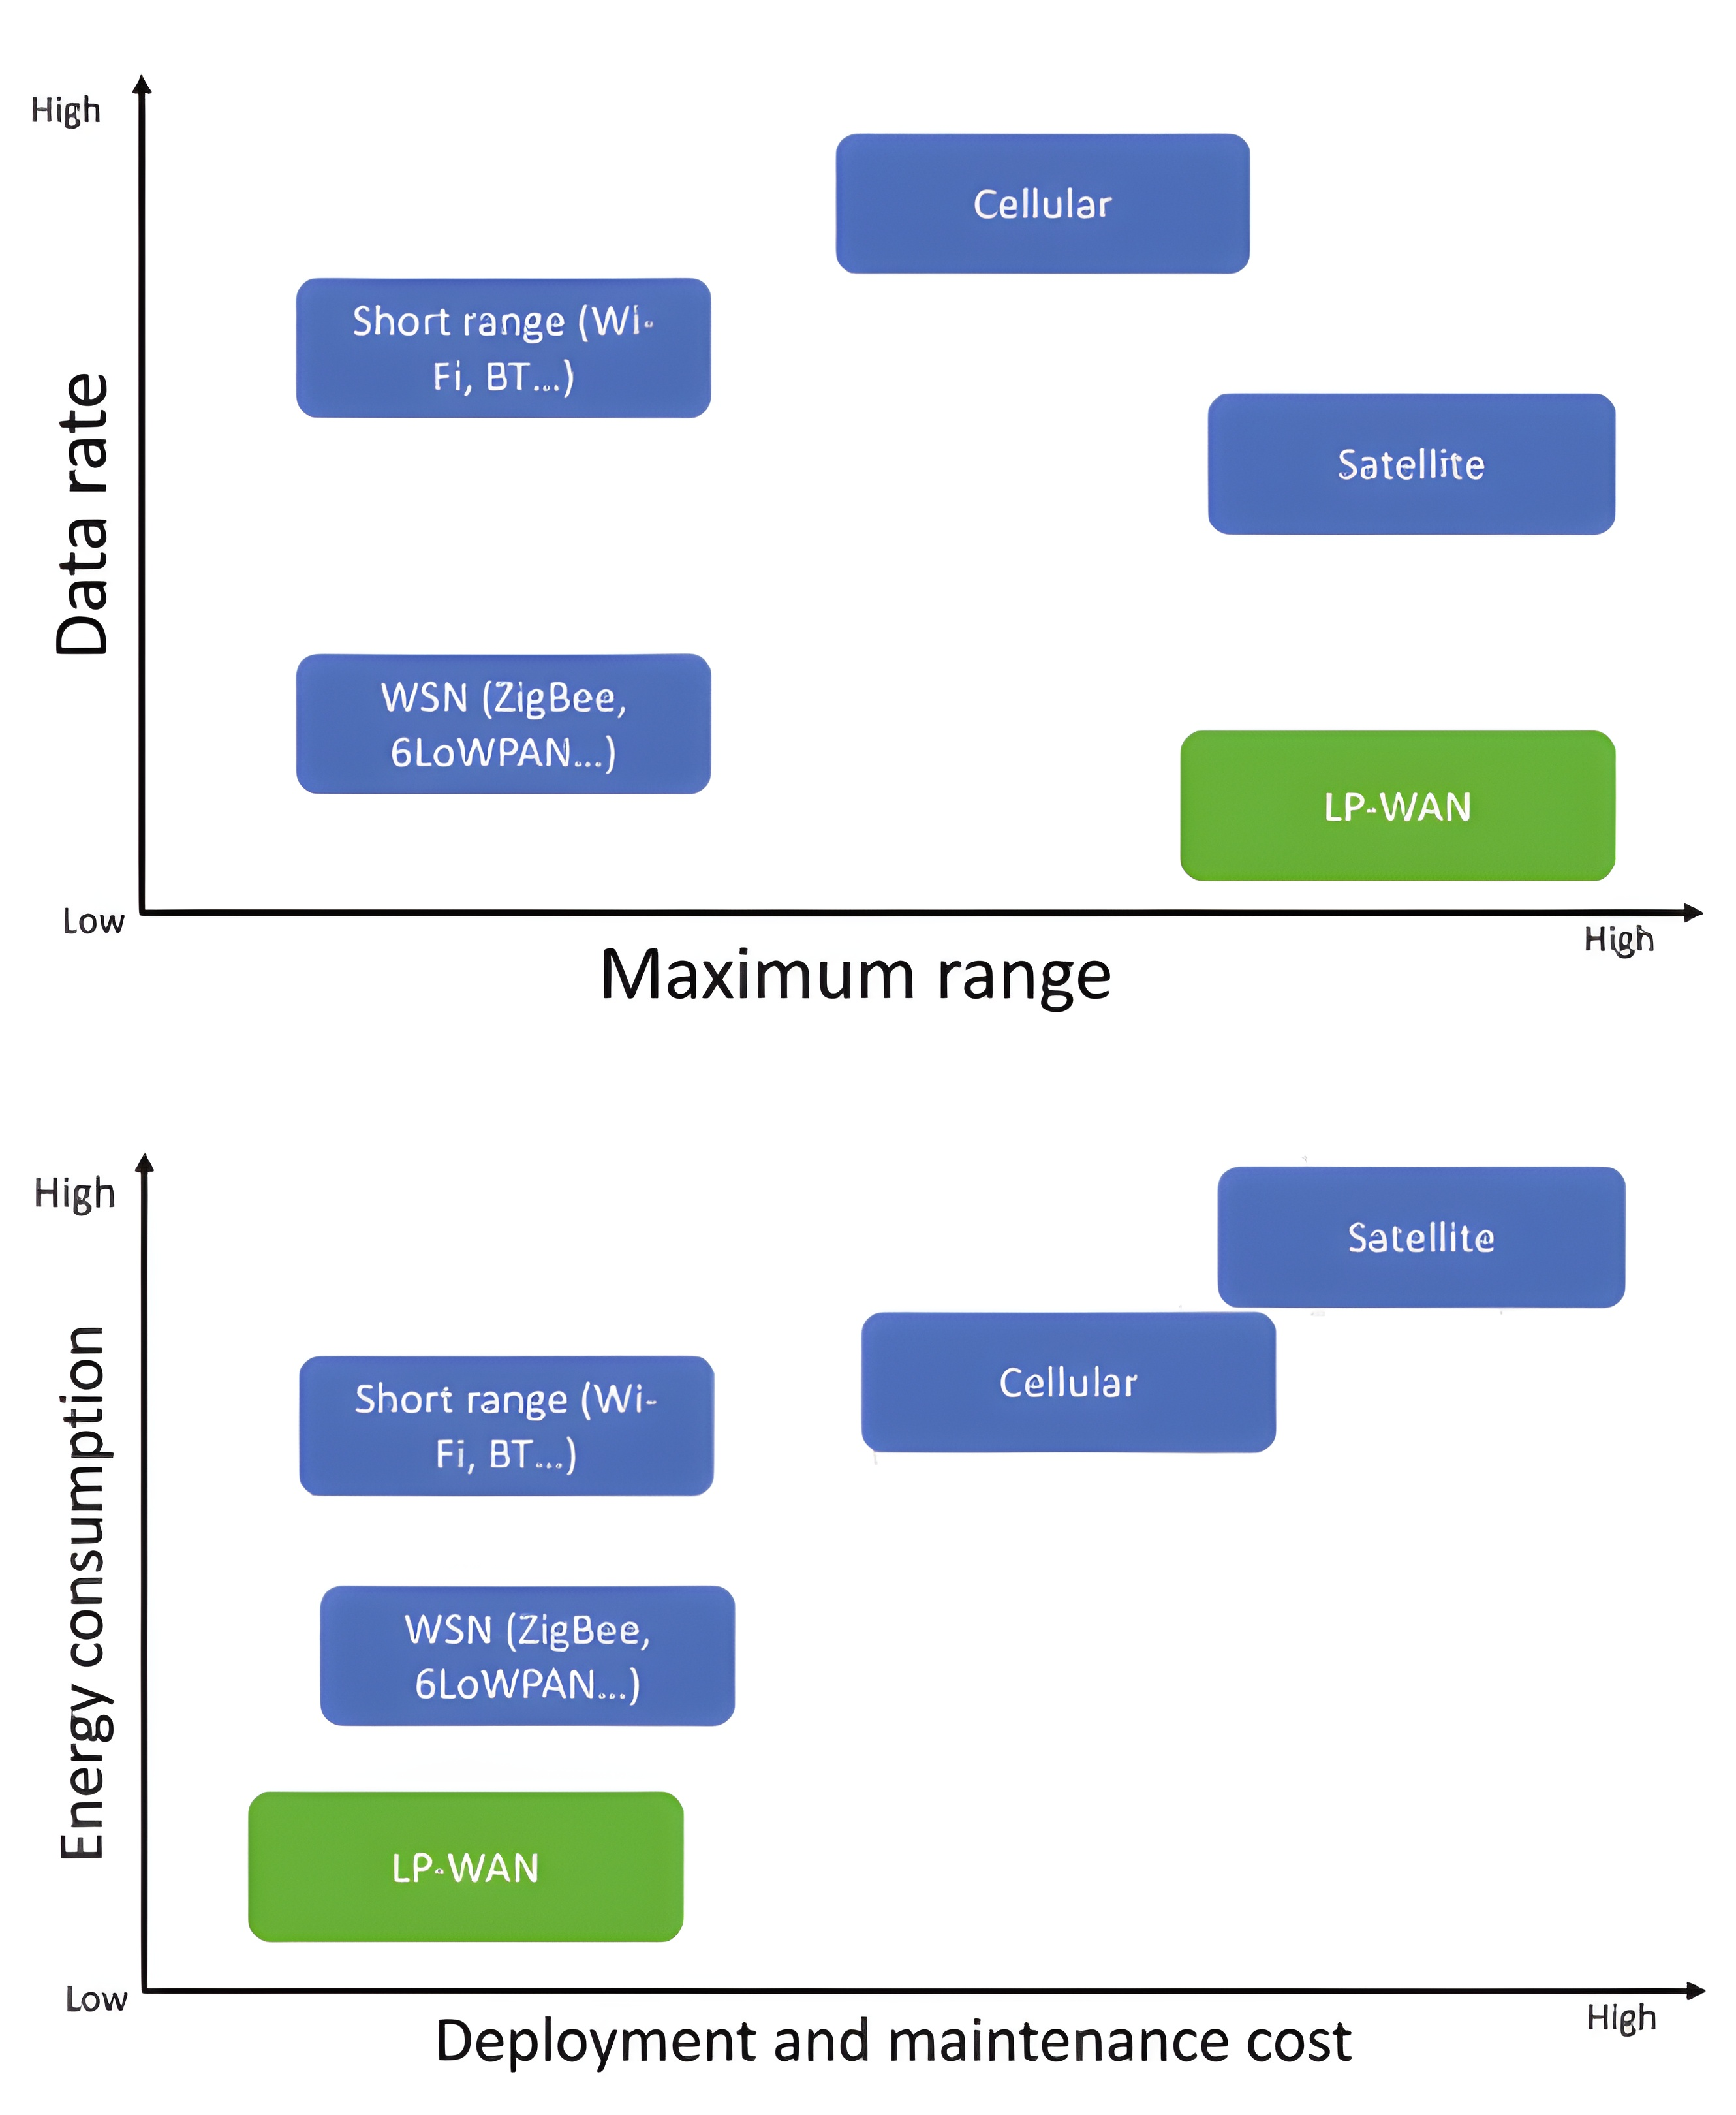
\includegraphics[scale=0.1]{Sections/Introduction/LP-WAN-Range.jpg}
\end{figure}
\end{comment}



